\section{Requirements} 

	The product receives EEG/MEG sensor data and constructs a real-time 3D visualization of the brain's current activity.
	Users can choose between further options, changing the output immediately to their personal preferences.

\begin{figure}[h]

	\begin{center}
	
		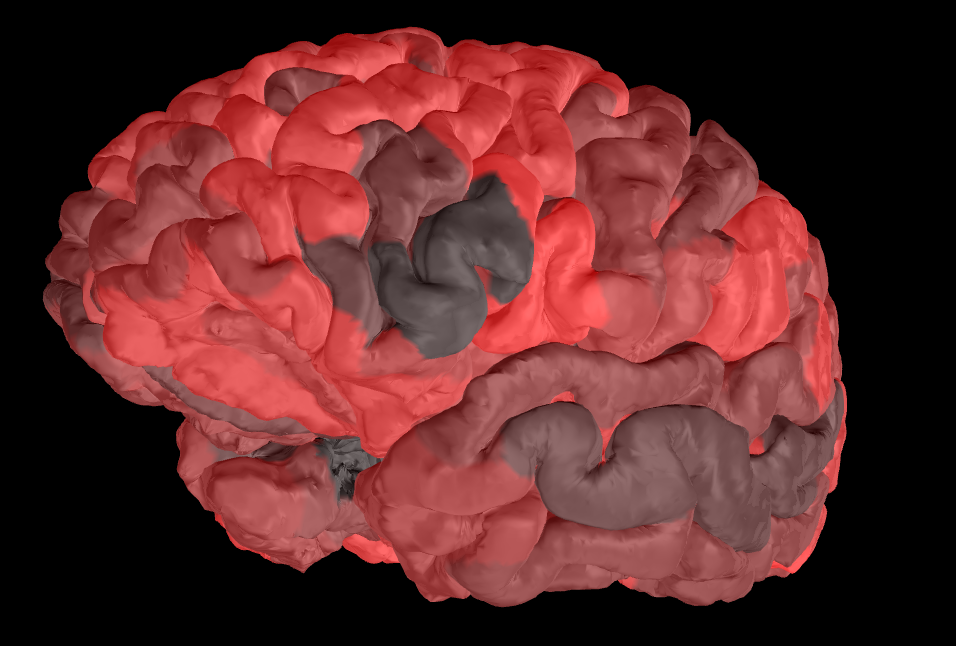
\includegraphics[scale=0.35]{Figures/disp3DScreenShot.png}
		\caption{Interpolated brain activity}
	
	\end{center}
	

\end{figure}

\subsection{Mandatory Criteria}

	The following functions have to be implemented correctly and must fulfill given requirements.
		
\subsubsection{Surface Constrained Distance Calculation (SCDC)} \label{scdc}
	
	Because the algorithm is supposed to work on folded surfaces, e.g. the brain, a function for calculating the distance between two points is needed.
	
	As the euclidian distance would not respect the structure of the surface, a different approach for determining the exact 	distances has to be implemented.  
	The function receives input data in form of a preprocessed triangulated surface mesh and calculates the distance between 	the vertices.			
	
	
	\begin{aims}
	
		\item[C111] Based on a given mesh, the function calculates a matrix that holds values describing the distances between 						all vertices using double precision. 
		\item[C112] The function must be able to process up to 200,000 vertices.
		\item[C113] The user can limit the calculation to a subset of vertices. 
	
	\end{aims}

\subsubsection{Sensor-to-Mesh Mapping} \label{projection}

	Since the sensors do not directly touch the head and therefore float slightly above it, an accurate projection is needed 	to exactly localize their positions on the surface beneath (e.g. head/brain/MEG helmet). 
	
	Hence a function must be implemented to solve this problem. 
	The function receives a set of sensor locations in 3D-Space and maps them onto the underlying mesh. Thus every 			sensor gets assigned to a vertex of the mesh. 

	\begin{aims}
	
		\item[C121] The function must be able to handle data from MEG-sensors which have a known orientation.
		\item[C122] The function must be able to handle data from EEG-sensors which are non-orientated.
	
	\end{aims}

\subsubsection{Interpolation Algorithm} \label{interpolation} 

	The main task is the ongoing interpolation, processing a particular set of sensor data, representing the brain's 			activity.
	
	Because the number of vertices is bigger than the quantity of sensor points, most vertex-values must be interpolated.
	Thus the algorithm receives a mesh and a subset of vertices with their respective sensor data.  
	
	\begin{aims}
	
		\item[C131] Based on the said subset the algorithm must calculate the values of the neurophysiological activity for every vertex of the mesh.
		\item[C132] For this, the algorithm creates a matrix storing weights for the later interpolation.
					The interpolation process can be summarized by the following equation: 
					
					$y_{full} = W \cdot y_{sub}$
					, where $W$ is the mentioned matrix and $y_{sub}$ is the current dataset for the known sensors, i.e. 							vertices.
		\item[C133] The calculation of the weight matrix must be based on the result of the SCDC (\ref{scdc}).
		\item[C134] Bad channels, a part of the given sensor meta data, must be considered during processing. 
	
	\end{aims}

\subsubsection{Integration in Disp3D} \label{integration}
	
	In order to ensure usability within the given framework MNE-CPP, the final visualization must be integrated into the 			preexisting 3D visualization library, namely Disp3D.
	
	\begin{aims}
		
		\item[C141] A new function must be added to the Disp3D tree model. Internally this function must create a new 								handler. 
		
	\end{aims}
	
\subsubsection{Non-Functional Requirements}		
	
	
	\begin{aims}

		\item[C151] The software is cross-platform compatible. 						
		\item[C152] Features \ref{scdc} and \ref{projection} are implemented in the class \textit{GeometryInfo}, while 								\ref{interpolation} is facilitated in the class \textit{Interpolation}.
		\item[C153] The function to integrate the product into Disp3D (\ref{integration}) is named \textit{addSensorData()}.
		\item[C154] For introduction purposes, a product video is to be created and published on the MNE-CPP website.  
		\item[C155] The software must be integratable into MNE Scan. 
		\item[C156] Only Qt libraries and the Eigen framework are used during development.
	
	\end{aims}
	
\newpage	
	
\subsection{Optional Criteria}
	
	As long as the mandatory requirements are fulfilled, it is desirable to further match the following criteria. 	
	
\subsubsection[SCDC]{SCDC (\ref{scdc})}
	
	\begin{aims}
		
		\item[C211] The computation time should be as low as possible.
		\item[C212] A threshold for the maximum distance between two vertices is used for reduction of processing time.
		
	\end{aims}
	
\subsubsection[Interpolation]{Interpolation (\ref{interpolation})}

	\begin{aims}
	
		\item[C221] One interpolation cycle should take less than 17ms.
		\item[C222] Multiple methods for calculating the weight matrix can be implemented. The user can select one.
		\item[C223] The computation is executed on GPU-level using compute shaders.
	
	\end{aims}
	
	
\subsection{Delimiting Criteria} 
	
	The following criteria limit the functionality of the system.
	
	\begin{aims}
		
		\item[C311] The program receives preprocessed data and does not get in touch with hardware sensors.
		\item[C312] The program does not evaluate the data medically and solely processes the data for further 										visualization. 						
		
	\end{aims}
	



	
